\documentclass{article}

\usepackage{graphicx}
\usepackage{tikz}
\usepackage{tikzsymbols}
\usetikzlibrary{calc,patterns,shapes.geometric}
\pagestyle{empty}
\usepackage[margin=0pt]{geometry}
\geometry{papersize={14in,12in}}

\def\centerarc[#1](#2)(#3:#4:#5){\draw[#1] ($(#2)+({#5*cos(#3)},{#5*sin(#3)})$) arc (#3:#4:#5);}

\begin{document}
	\begin{figure}
		\centering
		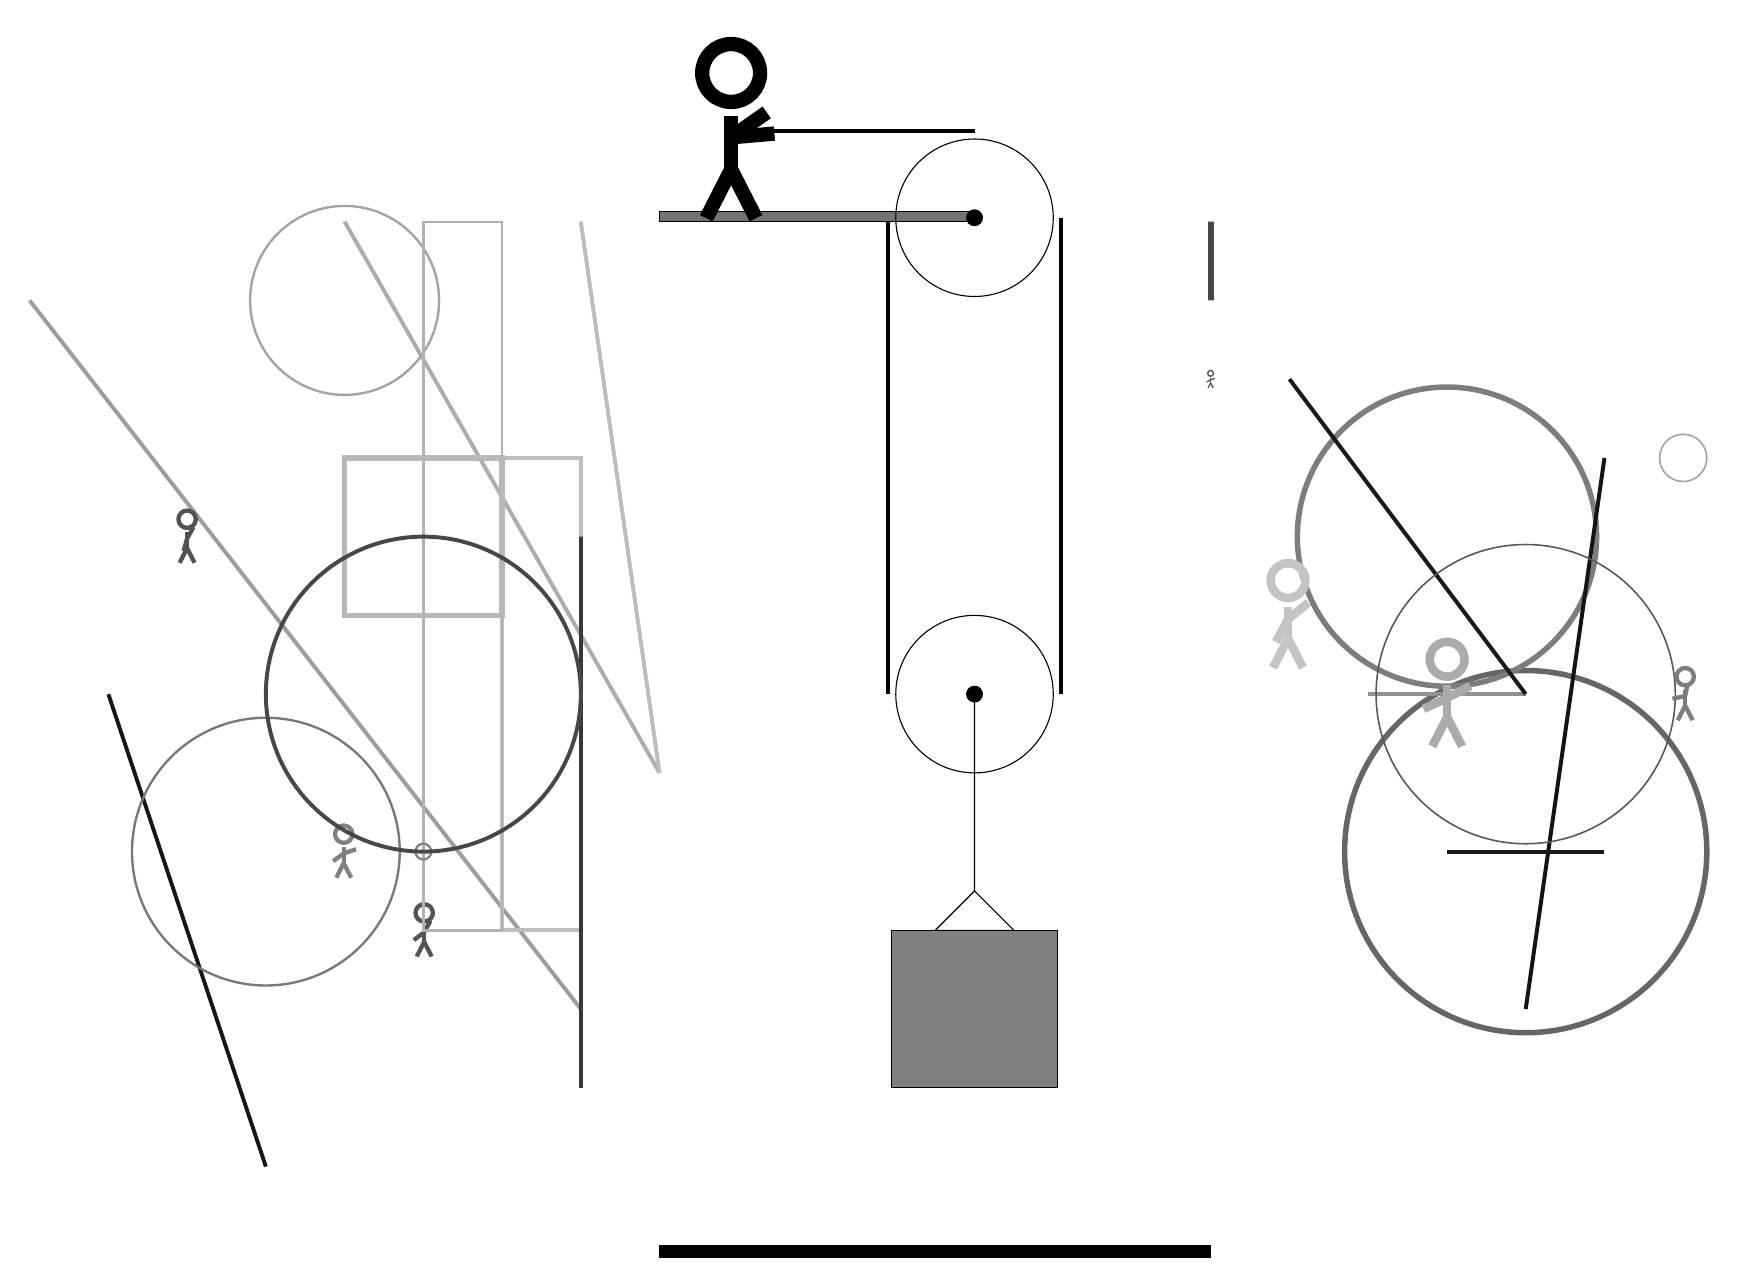
\begin{tikzpicture}
			%%%%% START %%%%%
			
			\draw[fill=black!55] (-2, 10) rectangle (2, 10.125);
			
			\draw (2, 4.0) circle (1);
			\draw[fill=black] (2, 4.0) circle (0.1);
			
			\draw (2, 10.05) circle (1);
			\draw[fill=black] (2, 10.05) circle (0.1);
			
			\draw (2, 4.0) -- (2, 1.5) -- (1.5, 1.0) -- (2.5, 1.0) -- (2, 1.5);
			\draw[fill=black!50] (0.95, 1.0) rectangle (3.05, -1.0);
			
			\draw[line width=0.5mm] (0.9, 10) -- (0.9, 4.0);
			\centerarc[line width=0.5mm](2, 4.0)(180:360:1.1);
			\draw[line width=0.5mm](3.1, 4.0) -- (3.1, 10.05);
			\centerarc[line width=0.5mm](2, 10.05)(0:90:1.1);
			\draw[line width=0.5mm](2, 11.15) -- (-1, 11.15);
			
			\node at (-1, 11.15) {\Strichmaxerl[10][-175][35]};
			
			\draw [line width=0.7mm, color=black!60](9, 2) circle (2.3);
			
			\node[line width=0.6mm, color=black!64] at (5, 8) {\Strichmaxerl[1][29][18]};
			\draw [line width=0.7mm, color=black!51](8, 6) circle (1.9);
			\draw[line width=0.5mm, color=black!92](9, 0) -- (10, 7);
			\draw[line width=0.5mm, color=black!38](-3, 0) -- (-10, 9);
			\draw[line width=0.5mm, color=black!43](7, 4) -- (9, 4);
			\node[line width=0.5mm, color=black!50] at (-6, 2) {\Strichmaxerl[3][36][19]};
			\draw[line width=0.5mm, color=black!32](-6, 10) -- (-2, 3);
			\draw[line width=0.5mm, color=black!25] (-4, 1) rectangle (-3, 7);
			
			\draw[line width=0.5mm, color=black!90](9, 4) -- (6, 8);
			\draw [line width=0.2mm, color=black!66](9, 4) circle (1.9);
			
			\draw[line width=0.5mm, color=black!78] (-3, -1) rectangle (-3, 6);
			\draw [line width=0.2mm, color=black!37](11, 7) circle (0.3);
			
			\draw[line width=0.7mm, color=black!72] (5, 10) rectangle (5, 9);
			\draw [line width=0.3mm, color=black!36](-6, 9) circle (1.2);
			\node[line width=0.3mm, color=black!67] at (-5, 1) {\Strichmaxerl[3][37][61]};
			\draw[line width=0.5mm, color=black!91](-7, -2) -- (-9, 4);
			
			\draw[line width=0.5mm, color=black!26](-3, 10) -- (-2, 3);
			\draw[line width=0.3mm, color=black!30] (-4, 1) rectangle (-5, 10);
			
			\node[line width=0.2mm, color=black!68] at (-8, 6) {\Strichmaxerl[3][74][61]};
			\draw[line width=0.7mm, color=black!28] (-4, 5) rectangle (-6, 7);
			
			\node[line width=0.7mm, color=black!51] at (11, 4) {\Strichmaxerl[3][12][79]};
			\draw [line width=0.3mm, color=black!48](-5, 2) circle (0.1);
			\draw [line width=0.3mm, color=black!53](-7, 2) circle (1.7);
			\draw[line width=0.5mm, color=black!90](10, 2) -- (8, 2);
			
			\node[line width=0.4mm, color=black!23] at (6, 5) {\Strichmaxerl[6][62][39]};
			\draw [line width=0.5mm, color=black!72](-5, 4) circle (2.0);
			\node[line width=0.7mm, color=black!33] at (8, 4) {\Strichmaxerl[6][25][27]};
			
			
			\draw[fill=black] (-2, -3) rectangle (5, -3.15);
			
			%%%%% END %%%%%
		\end{tikzpicture}
	\end{figure}	
\end{document}